\appendix

% ==============================================================
% A. PROOFS AND THEORETICAL DETAILS
% ==============================================================
\section{Proofs and Theoretical Details}
\label{app:theory}

This appendix provides proofs and additional details for the theoretical results in \cref{sec:method}.

% Section A.1
% --------------------------------------------------------------
\subsection{Failure-Set Nesting}
\label{app:failure-nesting}

For thresholds $\gamma_1<\gamma_2$, the corresponding failure sets are nested as
\[
    \{x:\rho(x)\leq\gamma_1\}
    \subseteq
    \{x:\rho(x)\leq\gamma_2\}.
\]
The associated conditional input distributions satisfy
\[
    p(x\mid\rho(x)\leq\gamma_1)
    =
    \frac{
        p(x\mid\rho(x)\leq\gamma_2)
        \mathds{1}\{\rho(x)\leq\gamma_1\}
    }{
        P\!\left(
            \rho(X)\leq\gamma_1
            \mid
            \rho(X)\leq\gamma_2
        \right)
    }.
\]

\begin{proof}
Starting from the right-hand side,
\[
\begin{aligned}
\frac{
    p(x\mid\rho(x)\leq\gamma_2)
    \mathds{1}\{\rho(x)\leq\gamma_1\}
}{
    P(
        \rho(X)\leq\gamma_1
        \mid
        \rho(X)\leq\gamma_2
    )
}
&=
\frac{
    p(x)
    \mathds{1}\{\rho(x)\leq\gamma_2\}
    \mathds{1}\{\rho(x)\leq\gamma_1\}
}{
    P(\rho(X)\leq\gamma_2)
    P(
        \rho(X)\leq\gamma_1
        \mid
        \rho(X)\leq\gamma_2
    )
}.
\end{aligned}
\]
Because $\gamma_1<\gamma_2$,
\[
    \mathds{1}\{\rho(x)\leq\gamma_2\}
    \mathds{1}\{\rho(x)\leq\gamma_1\}
    =
    \mathds{1}\{\rho(x)\leq\gamma_1\}
\]
and
\[
    P(\rho(X)\leq\gamma_2)
    P(
        \rho(X)\leq\gamma_1
        \mid
        \rho(X)\leq\gamma_2
    )
    =
    P(\rho(X)\leq\gamma_1).
\]
Therefore,
\[
    \frac{
        p(x)\mathds{1}\{\rho(x)\leq\gamma_1\}
    }{
        P(\rho(X)\leq\gamma_1)
    }
    =
    p(x\mid\rho(x)\leq\gamma_1),
\]
which proves the result.
\end{proof}

% Section A.2
% --------------------------------------------------------------
\subsection{Smoothed Observation Model}
\label{app:smoothed-observation}

Because $R=\rho(X)$ is deterministic given $X$, the joint distribution of $(X,R)$ is supported on the graph $\{(x,\rho(x))\}$ and is singular with respect to Lebesgue measure on $\mathcal X\times\mathbb R$. For $\sigma>0$, define the noisy robustness observation
\[
    \tilde R
    =
    \rho(X)+\varepsilon,
    \qquad
    \varepsilon\sim\mathcal N(0,\sigma^2).
\]
Its joint density with $X$ is
\[
    \tilde p_\sigma(x,r)
    =
    p(x)k_\sigma(r-\rho(x)),
\]
where $k_\sigma$ is the Gaussian density with standard deviation $\sigma$.

\paragraph{Well-posedness.}
For every $\sigma>0$, $\tilde p_\sigma$ is an absolutely continuous probability density on $\mathcal X\times\mathbb R$. Moreover, its marginal density over $x$ is the nominal input density $p(x)$.
\vspace{0.3cm}

\begin{proof}
Nonnegativity follows from nonnegativity of $p$ and $k_\sigma$. Integrating over both variables gives
\[
\begin{aligned}
    \int_{\mathcal X}\int_{\mathbb R}
    \tilde p_\sigma(x,r)\,dr\,dx
    &=
    \int_{\mathcal X}
    p(x)
    \left[
        \int_{\mathbb R}
        k_\sigma(r-\rho(x))\,dr
    \right]dx \\
    &=
    \int_{\mathcal X}p(x)\,dx \\
    &=1.
\end{aligned}
\]
Similarly,
\[
    \int_{\mathbb R}
    \tilde p_\sigma(x,r)\,dr
    =
    p(x)
\]
because the Gaussian kernel integrates to one.
\end{proof}

Marginalizing the smoothed density over the sublevel set $r\leq\gamma$ gives
\[
\begin{aligned}
    \int_{-\infty}^{\gamma}
    \tilde p_\sigma(x,r)\,dr
    &=
    p(x)
    \int_{-\infty}^{\gamma}
    k_\sigma(r-\rho(x))\,dr \\
    &=
    p(x)
    \Phi\!\left(
        \frac{\gamma-\rho(x)}{\sigma}
    \right)
\end{aligned}
\]
where $\Phi$ is the standard normal cumulative distribution function. Thus, smoothing replaces the hard indicator $\mathds{1}\{\rho(x)\leq\gamma\}$ with the probit factor
\[
    \Phi\!\left(
        \frac{\gamma-\rho(x)}{\sigma}
    \right).
\]
For every $x$ such that $\rho(x)\neq\gamma$, this factor converges to $\mathds{1}\{\rho(x)\leq\gamma\}$ as $\sigma\to0$.

% Section A.3
% --------------------------------------------------------------
\subsection{Convergence of the Smoothed Target}
\label{app:smoothing-convergence}

\begin{proposition}
\label{prop:smoothing-convergence}
Fix a threshold $\gamma$ such that
\[
    F_\rho(\gamma)
    =
    P(R\leq\gamma)
    >
    0.
\]
Assume there exists $\delta>0$ such that $R=\rho(X)$ admits a density $f_\rho$ on $I_\delta:=(\gamma-\delta,\gamma+\delta)$ that is bounded on $I_\delta$ and continuous at $\gamma$. No global density, boundedness, or continuity of $f_\rho$ is assumed. Outside $I_\delta$, the distribution of $R$ is arbitrary.

Define
\[
    h_\sigma(r)
    =
    \Phi\!\left(
        \frac{\gamma-r}{\sigma}
    \right),
    \qquad
    Z_\sigma
    =
    \mathbb E[h_\sigma(R)].
\]
The normalized smoothed target is
\[
    q_\sigma^\gamma(x)
    =
    \frac{
        p(x)h_\sigma(\rho(x))
    }{
        Z_\sigma
    },
\]
while the hard conditional target is
\[
    q^{*\gamma}(x)
    =
    \frac{
        p(x)\mathds{1}\{\rho(x)\leq\gamma\}
    }{
        F_\rho(\gamma)
    }.
\]
Then, as $\sigma\to0$,
\[
    \operatorname{TV}
    \left(
        q_\sigma^\gamma,
        q^{*\gamma}
    \right)
    =
    \frac{\sigma}{\sqrt{2\pi}}
    \lambda_\rho(\gamma)
    +
    o(\sigma),
    \qquad
    \lambda_\rho(\gamma)
    =
    \frac{
        f_\rho(\gamma)
    }{
        F_\rho(\gamma)
    }.
\]
Thus, if $f_\rho(\gamma)>0$,
\[
    \operatorname{TV}
    \left(
        q_\sigma^\gamma,
        q^{*\gamma}
    \right)
    =
    \frac{\sigma}{\sqrt{2\pi}}
    \lambda_\rho(\gamma)
    \bigl(1+o(1)\bigr).
\]
If $f_\rho(\gamma)=0$, the conclusion is instead
\[
    \operatorname{TV}
    \left(
        q_\sigma^\gamma,
        q^{*\gamma}
    \right)
    =
    o(\sigma).
\]
The multiplicative form does not apply in this case: whenever $P(R>\gamma)>0$, $q_\sigma^\gamma$ assigns positive mass above $\gamma$ for every $\sigma>0$, whereas $q^{*\gamma}$ does not.
\end{proposition}

\vspace{0.3cm}
\begin{proof}
Write $F=F_\rho(\gamma)$ and
\[
    H_\gamma(r)
    =
    \mathds{1}\{r\leq\gamma\}.
\]
Because both targets are absolutely continuous with respect to the nominal distribution of $X$, with Radon--Nikodym derivatives depending on $x$ only through $\rho(x)$,
\[
    \operatorname{TV}
    \left(
        q_\sigma^\gamma,
        q^{*\gamma}
    \right)
    =
    \frac{1}{2}
    \mathbb E
    \left|
        \frac{h_\sigma(R)}{Z_\sigma}
        -
        \frac{H_\gamma(R)}{F}
    \right|.
\]
Moreover,
\begin{equation}
\label{eq:tv-normalization-split}
    \left|
        2\operatorname{TV}
        \left(
            q_\sigma^\gamma,
            q^{*\gamma}
        \right)
        -
        \frac{1}{F}
        \mathbb E
        \left|
            h_\sigma(R)-H_\gamma(R)
        \right|
    \right|
    \leq
    \frac{|Z_\sigma-F|}{F}.
\end{equation}
It therefore suffices to expand the unnormalized $L^1$ error and show that $Z_\sigma-F=o(\sigma)$.

Let
\[
    g(u)
    =
    \Phi(-u)
    -
    \mathds{1}\{u\leq0\},
\]
so that
\[
    h_\sigma(r)-H_\gamma(r)
    =
    g\!\left(
        \frac{r-\gamma}{\sigma}
    \right).
\]
The kernel satisfies
\[
    |g(u)|
    =
    \Phi(-|u|),
    \qquad
    \int_{\mathbb R}|g(u)|\,du
    =
    \sqrt{\frac{2}{\pi}},
\]
and, by antisymmetry,
\[
    \int_{-A}^{A}g(u)\,du
    =
    0
    \qquad
    \text{for every }A>0.
\]

For any measurable $\psi$ with $|\psi(u)|\leq\Phi(-|u|)$, split the expectation into $R\in I_\delta$ and $R\notin I_\delta$. On $I_\delta$, the change of variables $r=\gamma+\sigma u$ gives
\[
    \mathbb E
    \left[
        \psi\!\left(
            \frac{R-\gamma}{\sigma}
        \right)
        \mathds{1}\{R\in I_\delta\}
    \right]
    =
    \sigma
    \int_{|u|<\delta/\sigma}
    \psi(u)
    f_\rho(\gamma+\sigma u)\,du.
\]
Continuity of $f_\rho$ at $\gamma$, boundedness on $I_\delta$, and integrability of $\psi$ then give
\[
    \sigma
    \int_{|u|<\delta/\sigma}
    \psi(u)f_\rho(\gamma+\sigma u)\,du
    =
    \sigma f_\rho(\gamma)
    \int_{|u|<\delta/\sigma}\psi(u)\,du
    +
    o(\sigma).
\]
Outside $I_\delta$,
\[
    \left|
        \psi\!\left(
            \frac{R-\gamma}{\sigma}
        \right)
    \right|
    \leq
    \Phi(-\delta/\sigma),
\]
so the tail contribution is superpolynomially small.

Taking $\psi=|g|$ therefore gives
\[
    \mathbb E
    \left|
        h_\sigma(R)-H_\gamma(R)
    \right|
    =
    \sigma f_\rho(\gamma)
    \sqrt{\frac{2}{\pi}}
    +
    o(\sigma).
\]
Taking $\psi=g$ and using $\int_{-\delta/\sigma}^{\delta/\sigma}g(u)\,du=0$ gives
\[
    Z_\sigma
    =
    F_\rho(\gamma)
    +
    o(\sigma).
\]
Substituting these expressions into \eqref{eq:tv-normalization-split} gives
\[
    \operatorname{TV}
    \left(
        q_\sigma^\gamma,
        q^{*\gamma}
    \right)
    =
    \frac{\sigma f_\rho(\gamma)}
         {\sqrt{2\pi}F_\rho(\gamma)}
    +
    o(\sigma)
    =
    \frac{\sigma}{\sqrt{2\pi}}
    \lambda_\rho(\gamma)
    +
    o(\sigma).
\]
The stated cases for $f_\rho(\gamma)>0$ and $f_\rho(\gamma)=0$ follow immediately.
\end{proof}

This is a fixed-threshold statement about the target distribution. It does not establish convergence of a fitted conditional proposal or justify a particular adaptive schedule for $\sigma$; proposal approximation error is separate from the smoothing error characterized above.

% Section A.4
% --------------------------------------------------------------
\subsection{Unbiasedness Under Adaptive Proposals}
\label{app:adaptive-unbiasedness}

We next establish unbiasedness for proposal-of-origin importance sampling under adaptive proposal selection. This result applies to the batch estimator in \cref{eq:batch-is}. It does not establish unbiasedness of the adaptive balance-MIS estimator in \cref{eq:balance-mis-estimator}.

Let $\mathcal F_{k-1}$ denote the history available before iteration $k$, and suppose the proposal $q_X^{(k)}$ is $\mathcal F_{k-1}$-measurable. Conditional on this history, draw
\[
    X_{k,1},\ldots,X_{k,n_k}
    \overset{\mathrm{iid}}{\sim}
    q_X^{(k)}.
\]
For a fixed evaluation threshold $\gamma$, define
\[
    \widehat P_k(\gamma)
    =
    \frac{1}{n_k}
    \sum_{i=1}^{n_k}
    \frac{
        p(X_{k,i})
    }{
        q_X^{(k)}(X_{k,i})
    }
    \mathds{1}\{
        \rho(X_{k,i})\leq\gamma
    \}.
\]
Assume $q_X^{(k)}(x)>0$ whenever $p(x)\mathds{1}\{\rho(x)\leq\gamma\}>0$, then $\mathbb E[\widehat P_k(\gamma)\mid\mathcal F_{k-1}]=P(\rho(X)\leq\gamma).$
\vspace{0.3cm}

\begin{proof}
Conditional on $\mathcal F_{k-1}$, the proposal $q_X^{(k)}$ is fixed. Therefore, for each sample,
\[
\begin{aligned}
    &
    \mathbb E
    \left[
        \frac{
            p(X_{k,i})
        }{
            q_X^{(k)}(X_{k,i})
        }
        \mathds{1}\{
            \rho(X_{k,i})\leq\gamma
        \}
        \,\middle|\,
        \mathcal F_{k-1}
    \right]
    \\
    &\qquad=
    \int
    q_X^{(k)}(x)
    \frac{
        p(x)
    }{
        q_X^{(k)}(x)
    }
    \mathds{1}\{
        \rho(x)\leq\gamma
    \}\,dx \\
    &\qquad=
    P(\rho(X)\leq\gamma).
\end{aligned}
\]
Averaging over the $n_k$ samples preserves the same conditional expectation. Taking expectation over $\mathcal F_{k-1}$ then gives
\[
    \mathbb E[
        \widehat P_k(\gamma)
    ]
    =
    P(\rho(X)\leq\gamma).
\]
\end{proof}

The result also holds for any deterministic weighted average of such batch estimators whose weights do not depend on the realized samples. In particular, averaging proposal-of-origin batch estimates across adaptive iterations remains unbiased. Proposal parameters, intermediate thresholds, and other adaptation choices may depend arbitrarily on the preceding history, provided that they are fixed before drawing the current batch and the support condition above holds.

The pooled balance-MIS estimator used by the amortized method has a different dependence structure. Its denominator contains proposals fitted using earlier samples, while later proposals may themselves depend on those samples. Consequently, the standard fixed-proposal balance-heuristic argument does not directly imply unbiasedness in this adaptive setting. We therefore use balance-MIS as the pooled estimator described in \cref{sec:alg-desc} without making an unbiasedness claim for that adaptive pooled construction.

% Section A.5
% --------------------------------------------------------------
\subsection{Defensive-Mixture Variance Bound}
\label{app:defensive-bound}

Let
\[
    q_\eta(x)
    =
    (1-\eta)q_X(x)+\eta p(x),
    \qquad
    0<\eta\leq1.
\]
Because $q_\eta(x)\geq\eta p(x)$, the corresponding importance weight satisfies
\[
    w_\eta(x)
    =
    \frac{
        p(x)
    }{
        q_\eta(x)
    }
    \leq
    \frac{1}{\eta}.
\]

For the event
\(
    F_\gamma
    =
    \{x:\rho(x)\leq\gamma\},
\)
let
\(
    P_\gamma
    =
    P(X\in F_\gamma).
\)
For one draw $X\sim q_\eta$, define
\[
    Y
    =
    w_\eta(X)
    \mathds{1}\{X\in F_\gamma\}.
\]
Then
\[
\begin{aligned}
    \mathbb E_{q_\eta}[Y^2]
    &=
    \mathbb E_{q_\eta}
    \left[
        w_\eta(X)^2
        \mathds{1}\{X\in F_\gamma\}
    \right] \\
    &\leq
    \frac{1}{\eta}
    \mathbb E_{q_\eta}
    \left[
        w_\eta(X)
        \mathds{1}\{X\in F_\gamma\}
    \right] \\
    &=
    \frac{P_\gamma}{\eta}.
\end{aligned}
\]
For the ordinary importance-sampling estimator based on $M$ independent draws from $q_\eta$,
\[
    \widehat P_\eta
    =
    \frac{1}{M}
    \sum_{i=1}^{M}
    w_\eta(X_i)
    \mathds{1}\{X_i\in F_\gamma\},
\]
we therefore have
\[
\begin{aligned}
    \operatorname{Var}(\widehat P_\eta)
    &=
    \frac{1}{M}
    \operatorname{Var}(Y) \\
    &\leq
    \frac{1}{M}
    \left(
        \frac{P_\gamma}{\eta}
        -
        P_\gamma^2
    \right) \\
    &\leq
    \frac{P_\gamma}{\eta M}.
\end{aligned}
\]
Thus, the defensive component guarantees both the pointwise weight bound $w_\eta(x)\leq1/\eta$ and a finite upper bound on the variance of the single-proposal importance-sampling estimator.

% ==============================================================
% B. EXPERIMENTAL PROBLEMS
% ==============================================================
\section{Experimental Problems}
\label{app:problems}

This appendix defines the benchmark problems used in the canonical experiments and gives the corresponding reference failure probabilities where available.

% Section B.1
% --------------------------------------------------------------
\subsection{Unimodal Gaussian Benchmark}
\label{app:unimodal}

Let $X\sim\mathcal N(0,I_2)$ and define
\(
    \rho(x)
    =
    3-\min(x_1,x_2).
\)
At threshold $\gamma$, failure occurs when $\rho(x)\leq\gamma$, or equivalently when
\[
    x_1\geq3-\gamma,
    \qquad
    x_2\geq3-\gamma.
\]
Because the coordinates are independent, 
\[
    P(\rho(X)\leq\gamma) = \Phi\!\left(-(3-\gamma)\right)^2.
\]
At $\gamma=0$,
\[
    P(\rho(X)\leq0)
    =
    \Phi(-3)^2
    \approx
    1.8222\times10^{-6}.
\]

This benchmark has a single connected failure region and is used to evaluate the benefit of amortizing proposal learning as the number of requested thresholds increases.

% Section B.2
% --------------------------------------------------------------
\subsection{Radial Shell}
\label{app:shell}

Let $X\sim\mathcal N(0,I_d)$ and define $\rho(x)=r_c-\|x\|.$ Then $\rho(x)\leq\gamma$ if and only if $\|x\|\geq r_c-\gamma.$ Since
\[
    \|X\|^2\sim\chi_d^2,
\]
the failure-probability curve is
\[
    P(\rho(X)\leq\gamma)
    =
    P\!\left(
        \chi_d^2
        \geq
        (r_c-\gamma)^2
    \right).
\]

We evaluate $d\in\{2,20\}$. For each dimension, the evaluation grid contains 16 thresholds whose exact failure probabilities are logarithmically spaced from $10^{-3}$ to $10^{-6}$. The smallest threshold is $\gamma_{\min}=0.5$, and $r_c$ is chosen so that this threshold corresponds to the rarest grid point. This gives
\[
    r_c
    =
    5.756521769751461
    \qquad
    \text{for }d=2,
\]
and
\[
    r_c
    =
    8.588305201645746
    \qquad
    \text{for }d=20.
\]

Unlike the unimodal benchmark, the shell has no distinguished failure direction: equal-robustness sets are spheres. It therefore tests whether the adaptive sampler can discover an extended isotropic rare-event region rather than a localized failure mode.

% Section B.3
% --------------------------------------------------------------
\subsection{Multimodal Tail Benchmark}
\label{app:tail-race}

Let $X\sim\mathcal N(0,I_2)$ and define
\(
    \rho(x)
    =
    \min\!\left(
        c_1-x_1,\,
        c_2-x_2^2
    \right).
\)
We fix $c_1=5.5$ and evaluate \[c_2\in\{16,18,20,23\}.\]

At threshold $\gamma$, failure occurs if either $x_1\geq c_1-\gamma$ or $|x_2|\geq\sqrt{c_2-\gamma}$, for thresholds satisfying $c_2-\gamma\geq0$. Define
\[
    P_1(\gamma)
    =
    \Phi(\gamma-c_1)
\]
and
\[
    P_2(\gamma)
    =
    2\Phi\!\left(
        -\sqrt{c_2-\gamma}
    \right).
\]
By independence,
\[
    P(\rho(X)\leq\gamma)
    =
    P_1(\gamma)
    +
    P_2(\gamma)
    -
    P_1(\gamma)P_2(\gamma).
\]

At the target threshold $\gamma=0$, the four settings have failure probabilities
\[
\begin{aligned}
    c_2=16 &: \quad 6.3361\times10^{-5},\\
    c_2=18 &: \quad 2.2109\times10^{-5},\\
    c_2=20 &: \quad 7.7632\times10^{-6},\\
    c_2=23 &: \quad 1.6390\times10^{-6}.
\end{aligned}
\]

The first failure mechanism produces a one-sided tail in $x_1$, while the second produces upper and lower tails in $x_2$, yielding three failure lobes. The $x_1$ lobe has probability $\Phi(-c_1)=1.90\times10^{-8}$ independently of $c_2$, so the two $x_2$ lobes carry $99.97\%$, $99.91\%$, $99.76\%$ and $98.84\%$ of the failure probability at $c_2=16,18,20,23$. Varying $c_2$ therefore does not move the dominant mechanism; it moves the two dominant lobes progressively further into the tail, from $|x_2|\geq 4.00$ to $|x_2|\geq 4.80$, while the easily reached but nearly massless $x_1$ lobe stays fixed. This is the sense in which the important input modes vary with robustness, and it motivates using the benchmark to test whether the conditioned method discovers and retains these modes more consistently than the unconditional baseline.

The conditioned and unconditional methods differ in one additional implementation detail beyond robustness conditioning. The conditioned method fits its proposal using the accumulated sample buffer, whereas the unconditional cross-entropy baseline fits using elites from the current batch. This difference can improve retention of modes once they have been discovered. We therefore use this experiment to compare the full conditioned method against the unconditional baseline, rather than to isolate the effect of conditioning alone.

% Section B.4
% --------------------------------------------------------------
\subsection{Autonomous-Driving Crosswalk}
\label{app:idm}

The high-dimensional benchmark is a closed-loop autonomous-driving crosswalk scenario with longitudinal vehicle control and stochastic pedestrian disturbances. The random input contains 30 decision steps with five disturbance channels per step, giving
\[
    d=150.
\]
The five channels consist of two pedestrian-acceleration components and three sensing-noise components. The channels enter the simulator as a $5\times30$ matrix; column $k$ is held constant over decision step $k$. The initial encounter geometry is deterministic---a $4.0\,\mathrm{m}\times1.8\,\mathrm{m}$ vehicle approaching at $8\,\mathrm{m/s}$ and a $1.0\,\mathrm{m}\times1.0\,\mathrm{m}$ pedestrian crossing at $1.5\,\mathrm{m/s}$---so all stochasticity is carried by the disturbance vector. The horizon is $30$ decision steps, that is $6.0\,\mathrm{s}$ of simulated time, terminating early on collision or on either agent leaving the scene.

The decision interval is
\[
    0.2\,\mathrm{s},
\]
and the simulator uses four physics substeps per decision interval, giving
\[
    \Delta t_{\mathrm{phys}}
    =
    0.05\,\mathrm{s}.
\]
The disturbance scale is
\[
    a_{\mathrm{scale}}
    =
    0.60.
\]

The simulator's per-step reward is $1$ on collision and $20/(\ell_t^2+20)$ otherwise, where $\ell_t$ is the Euclidean distance between the vehicle and pedestrian centres, evaluated once per physics substep. Robustness is defined from the running maximum of that reward,
\[
    \rho
    =
    0.99-\max_t r_t,
\]
so $\rho$ decreases as the closest approach over the trajectory decreases. Inverting the reward gives the corresponding minimum separation
\[
    \mathrm{sep}(\gamma)
    =
    \sqrt{20/(0.99-\gamma)-20}
\]
measured centre to centre. The constant $0.99$ is a benchmark constant placing the target just below the collision reward of $1$; it does not encode a physical clearance. Because the vehicle and pedestrian bounding boxes overlap at roughly $1.4\,\mathrm{m}$ centre-to-centre separation, the target event $\{\rho\leq0\}$ is realized in this scenario only by collisions. In the $26$-million-rollout reference, the same $808$ observed events satisfy both $\rho\leq0.08$ and $\rho\leq0$, and all have the collision value $\rho=-0.01$. The two thresholds are nevertheless mathematically distinct under the simulator definition.

The evaluation threshold grid is
\[
    \mathcal G
    =
    \{
        0.434,\,
        0.38,\,
        0.32,\,
        0.26,\,
        0.20,\,
        0.14,\,
        0.08,\,
        0
    \}.
\]

The comparison reference is constructed from $26$ million simulator rollouts using the same disturbance dimension, disturbance scale, physics time step, and robustness definition as the experimental runs. The reference configuration matches the experimental configuration in all recorded fields; the physics time step is additionally verified from the reference-generation source code. The resulting empirical failure-probability curve is used in \cref{sec:driving-results}. 

The reference is banked as a histogram of $\rho$ with bin width $5\times10^{-4}$ over $2{,}040$ bins, and the eight evaluation thresholds fall exactly on bin edges. We evaluate each threshold using the event $\rho\leq\gamma$. The corresponding event counts are $225{,}259$, $98{,}187$, $37{,}243$, $12{,}991$, $5{,}498$, $3{,}089$, $808$ and $808$ out of $26{,}000{,}000$. The resulting failure probabilities range from $8.6638\times10^{-3}$ at $\gamma=0.434$ to $3.1077\times10^{-5}$ at $\gamma=0$. Relative standard errors range from $0.21\%$ to $3.5\%$. The Wilson $95\%$ intervals are approximately $[8.628,8.700]\times10^{-3}$ at $\gamma=0.434$ and $[2.901,3.329]\times10^{-5}$ at $\gamma=0$. The two rarest thresholds contain the same $808$ observed reference events, although the thresholds are evaluated separately. The reference run was not seeded and is therefore not bit-reproducible; the banked histogram is the artifact of record.

% ==============================================================
% C. ADDITIONAL EXPERIMENTAL RESULTS
% ==============================================================
\section{Additional Experimental Results}
\label{app:additional-results}

This appendix reports supporting results and diagnostics for the experiments in \cref{sec:experiments}.

% Section C.1
% --------------------------------------------------------------
\subsection{Additional Amortization Results}
\label{app:additional-amortization}

\Cref{fig:exp1-additional-curves} shows representative probability curves for the smallest and largest numbers of requested thresholds in the amortization experiment. The plotted estimates are the raw finite positive importance-sampling estimates (missing estimates are not replaced by the $1/B$ convention used to compute ILE).

\Cref{tab:exp1-full-results} gives the corresponding aggregate results for all values of $m$. The amortized estimator maintains ILE near $0.015$ with complete coverage throughout the sweep, and the unconditional CEM baseline maintains ILE between $0.018$ and $0.019$, also with complete coverage at every $m$. The per-threshold baseline becomes less accurate as the fixed simulation budget is divided among more independent proposal fits, with median coverage decreasing to $55.5\%$ at $m=100$.

Because ILE assigns a finite value to missing estimates, we also evaluate sensitivity to this convention. \Cref{tab:exp1-floor-sensitivity} recomputes ILE using two fixed substitute values in addition to the primary $1/B$ convention. The amortized results are unchanged because every seed has complete coverage for every value of $m$. The per-threshold result becomes sensitive to the convention only after coverage begins to decrease.

\begin{figure}[ht!]
    \centering
    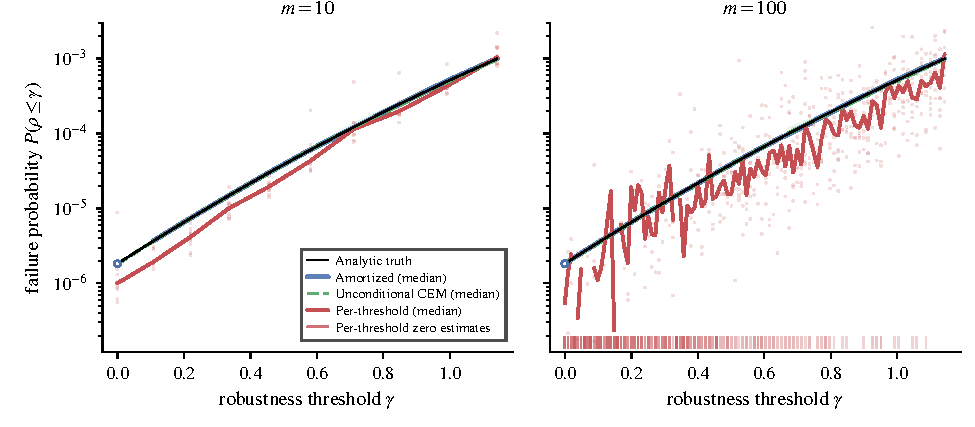
\includegraphics[width=0.9\linewidth]
        {figures/appendix/exp1_kscaling_curves.pdf}
    \caption{
    Representative failure-probability curves for the unimodal benchmark at \(m=10\) and \(m=100\) requested thresholds under the fixed total budget \(B=25{,}000\). The amortized and unconditional CEM medians closely track the analytic truth and therefore largely overlap visually, while the independently refitted per-threshold baseline becomes noisier and loses coverage at \(m=100\). Missing estimates are omitted rather than replaced by the \(1/B\) convention used for ILE.
    }
    \label{fig:exp1-additional-curves}
\end{figure}

\begin{table}[ht!]
    \centering
    \caption{
    Full-curve estimation as the number of requested thresholds increases under a fixed budget of $B=25{,}000$ robustness evaluations. ILE is computed over the full threshold grid, substituting $1/B$ only for missing, zero, or non-finite estimates. Coverage is the fraction of requested thresholds with a finite positive estimate. Values are medians over 10 seeds.
    }
    \label{tab:exp1-full-results}
    \begin{tabular}{@{}lrrr@{}}
        \toprule
        Method & $m$ & ILE & Coverage \\
        \midrule
        Amortized
            & 10  & 0.0146 & 100.0\% \\
            & 25  & 0.0151 & 100.0\% \\
            & 50  & 0.0152 & 100.0\% \\
            & 100 & 0.0149 & 100.0\% \\
        \midrule
        Unconditional CEM
            & 10  & 0.0177 & 100.0\% \\
            & 25  & 0.0184 & 100.0\% \\
            & 50  & 0.0190 & 100.0\% \\
            & 100 & 0.0190 & 100.0\% \\
        \midrule
        Per-threshold
            & 10  & 0.4628 & 100.0\% \\
            & 25  & 0.5385 & 100.0\% \\
            & 50  & 0.6768 & 96.0\% \\
            & 100 & 1.2000 & 55.5\% \\
        \bottomrule
    \end{tabular}
\end{table}

\begin{table}[ht!]
    \centering
    \caption{
    Sensitivity of integrated log-error to the value substituted for missing, zero, or non-finite estimates in the unimodal benchmark. Positive finite estimates are never clipped. The primary analysis uses the budget-resolution convention $1/B$, with $B=25{,}000$. Values are medians over 10 seeds.
    }
    \label{tab:exp1-floor-sensitivity}
    \begin{tabular}{@{}lrrrr@{}}
        \toprule
        Method & $m$ & $1/B$ & $10^{-6}$ & $10^{-8}$ \\
        \midrule
        Amortized
            & 10  & 0.0146 & 0.0146 & 0.0146 \\
            & 25  & 0.0151 & 0.0151 & 0.0151 \\
            & 50  & 0.0152 & 0.0152 & 0.0152 \\
            & 100 & 0.0149 & 0.0149 & 0.0149 \\
        \midrule
        Per-threshold
            & 10  & 0.4628 & 0.4628 & 0.4628 \\
            & 25  & 0.5385 & 0.5385 & 0.5385 \\
            & 50  & 0.6768 & 0.6502 & 0.7644 \\
            & 100 & 1.2000 & 1.6361 & 3.7036 \\
        \bottomrule
    \end{tabular}
\end{table}

% Section C.2
% --------------------------------------------------------------
\subsection{Multimodal Tail Benchmark Results}
\label{app:tail-benchmark-results}

\Cref{tab:tail-benchmark-results} gives the seed-level mode-discovery statistics underlying \cref{fig:conditioning-modes}. Both classifications are computed by the run itself; neither is assigned after the fact. A seed is classified as discovering all three lobes when at least one draw with $\rho(x)\leq 0$ falls in each of the one-sided $x_1$ tail and the two $x_2$ tails defined in \cref{app:tail-race}, counted over all $80{,}000$ pooled draws of the run. A seed is classified as amplified when the importance-weighted probability mass its estimate attributes to the two $x_2$ lobes exceeds $10\%$ of the true failure probability; because those lobes carry more than $98\%$ of that probability at every $c_2$, this is in practice a threshold on the accuracy of $\widehat P$, and it selects exactly the seeds with $\widehat P/P_{\mathrm{true}}>0.1$. A seed is classified as locked when no draw with $\rho(x)\leq 0$ falls in either $x_2$ tail. The two classifications are independent: neither implies the other, and 12 of the 18 amplified seeds discovered only two lobes. 

\begin{table}[ht!]
    \centering
    \caption{
    Mode discovery and probability estimation on the multimodal tail benchmark. ``All'' is the number of 10 seeds that discover all three failure lobes, and ``Ampl.'' is the number classified in the amplified regime. The final two columns report the median ratio between the estimated and true failure probability at $\gamma=0$. The unconditional aggregates at $c_2=16$, $18$, and $23$ each include one fallback-assisted run.
    }
    \label{tab:tail-benchmark-results}
    \begin{tabular}{@{}lrrrrrr@{}}
        \toprule
        & \multicolumn{2}{c}{Conditioned}
        & \multicolumn{2}{c}{Unconditional}
        & \multicolumn{2}{c}{$\widehat P/P$} \\
        $c_2$
        & All & Ampl.
        & All & Ampl.
        & Conditioned & Unconditional \\
        \midrule
        16 & 6/10 & 7/10 & 1/10 & 4/10 & 0.436  & 0.00837 \\
        18 & 3/10 & 3/10 & 0/10 & 1/10 & 0.00365 & 0.000887 \\
        20 & 5/10 & 2/10 & 0/10 & 0/10 & 0.00237 & 0.00182 \\
        23 & 1/10 & 1/10 & 0/10 & 0/10 & 0.0107  & 0.00848 \\
        \bottomrule
    \end{tabular}
\end{table}

The single-draw threshold is weak at the larger thresholds---under the nominal distribution alone, $80{,}000$ draws are expected to place $5.1$, $1.8$, $0.6$ and $0.1$ points beyond $|x_2|\geq\sqrt{c_2}$ for $c_2=16,18,20,23$. 

As a sensitivity analysis, and not as a redefinition of the reported metric, we recomputed the counts requiring at least five failing draws in each lobe rather than one: the conditioned counts become 4/10, 1/10, 0/10 and 0/10, and the unconditional counts become 0/10 at all four settings, for $c_2=16,18,20,23$ respectively. The values reported in \cref{tab:tail-benchmark-results} and \cref{fig:conditioning-modes} remain those of the single-draw criterion. Under the stricter criterion the conditioned method retains an advantage only at $c_2=16$ and $c_2=18$; in particular the 5/10 versus 0/10 difference at $c_2=20$ does not survive, so that difference is better read as transient contact with the $x_2$ lobes than as sustained representation of them.

The conditioned method improves mode discovery more consistently than it improves the final probability estimate. At every value of $c_2$, the conditioned method discovers all three lobes in more seeds than the unconditional baseline. It also enters the amplified regime more often overall ($13$ versus $5$ of $40$ seeds), although this gap is smaller than the discovery gap. Run-level regime labels depend on individual adaptive trajectories, so single-seed differences such as $1/10$ versus $0/10$ should not be interpreted. Both methods, however, retain substantial seed-to-seed variability at the target threshold. Because the conditioned method fits on the accumulated sample buffer while the unconditional baseline fits on elites from the current batch, part of the difference in mode retention may arise from this fitting-set difference rather than from conditioning alone. The results therefore support a narrower interpretation: the full conditioned method can improve access to and retention of rare-event modes, but it does not guarantee accurate estimation when the relevant tail modes remain poorly sampled.

\paragraph{Degenerate-fit sensitivity.}
One unconditional run in each of the $c_2=16$, $18$, and $23$ settings terminated because of a degenerate mixture fit and was completed using a targeted fallback verified not to alter known-good runs. These runs are retained as fallback-assisted. Restricting each affected aggregate to its nine clean runs changes the median $\widehat P/P$ from $0.00837$ to $0.00898$ at $c_2=16$, from $0.000887$ to $0.00114$ at $c_2=18$, and from $0.00848$ to $0.00849$ at $c_2=23$. None of the three fallback-assisted runs discovers all three lobes or reaches the amplified regime, so the clean-only all-three-lobe and amplification counts are $1/9$ and $4/9$ at $c_2=16$, $0/9$ and $1/9$ at $c_2=18$, and $0/9$ and $0/9$ at $c_2=23$, compared with $1/10$ and $4/10$, $0/10$ and $1/10$, and $0/10$ and $0/10$ in the reported aggregate. Retaining these runs therefore changes the unconditional rates only through the denominator, and the qualitative comparison is unchanged.

% Section C.3
% --------------------------------------------------------------
\subsection{High-Dimensional Driving Diagnostics}
\label{app:high-diagnostics}

The probability curves in \cref{fig:driving-curve} show that the amortized estimator produces finite positive estimates across the full driving evaluation grid. We report additional diagnostics here to distinguish adaptive-schedule reach, sampling of the target region, and estimator-weight concentration.

Across the 10 seeds, the smallest adaptive threshold reached by the amortized proposal has median $\gamma_{\min}=0.362$, with range $0.305\leq\gamma_{\min}\leq0.369$. The adaptive schedule reaches the target threshold $\gamma=0$ in no seed.

Schedule reach is distinct from estimator availability. All 10 seeds contain samples at or below $\gamma=0$, with 36 to 66 of the $25{,}000$ draws per seed taking the simulator's collision value $\rho=-0.01$. Because the pooled estimator reuses samples collected across the adaptive run, it produces a finite positive estimate at every evaluation threshold in all 10 seeds, despite the adaptive schedule itself never reaching the target.

The schedule stalls rather than descending gradually. In every seed, $\gamma^{(k)}$ falls from about $0.69$ to about $0.37$ within the first four batches and then shows little further progress. Estimator weights nevertheless become increasingly concentrated toward the rare tail. For the pooled balance-MIS estimator, the median effective-sample-size fraction over samples with $\rho\leq0.434$ is $0.0256$. In absolute terms, median effective sample size decreases from $201$ at $\gamma=0.434$ to $54.8$ near the terminal adaptive threshold and $5.8$ at $\gamma=0$. Despite this concentration, all 10 target-threshold estimates are finite and lie within a factor of $3.25$ of the reference probability.

Proposal-density evaluation adds substantial computation beyond simulator calls. For the original amortized runs, marginal-density evaluation and pooled re-indexing dominate wall-clock time. Because the corrected baseline reruns used different concurrency settings, we do not compare wall-clock times across methods. The reported evaluation budgets therefore measure simulator effort rather than total computational cost.

% ==============================================================
% D. REPRODUCIBILITY AND EXPERIMENTAL CONFIGURATION
% ==============================================================
\section{Reproducibility and Experimental Configuration}
\label{app:reproducibility}

All reported method and baseline runs use fixed random seeds and saved experiment configurations. The final repository release will include the source snapshot, configuration files, and experimental artifacts corresponding to the reported results. All experiments were run with Julia 1.12.6.

\begin{table}[ht!]
    \centering
    \small
    \caption{
    Configurations for the four reported experiments. \(B\) is the nominal robustness-evaluation budget; baseline counts may differ because oracle-tuning costs are charged. SGM denotes the structured Gaussian mixture used in the high-dimensional conditional proposal.
    }
    \label{tab:canonical-configurations}

    \begin{tabular}{@{}lrrrrll@{}}
        \toprule
        Experiment
        & $d$
        & $B$
        & Batch
        & Iter.
        & Proposal
        & Settings \\
        \midrule

        Amortization
        & 2
        & 25k
        & 1k
        & 25
        & Cond.\ EMGMM
        & $C=2,\ \alpha=0.2$ \\

        Radial shell
        & 2, 20
        & 25k, 50k
        & 1k
        & 25 / 50
        & Cond.\ EMGMM
        & $C=2,\ \alpha=0.2$ \\

        Multimodal tail
        & 2
        & 80k
        & 2k
        & 40
        & Cond.\ EMGMM
        & $C=3,\ \alpha=0.15$ \\

        Driving
        & 150
        & 25k
        & 1k
        & 25
        & Cond.\ SGM
        & $C=2,\ r=10,\ \alpha=0.2$ \\

        \bottomrule
    \end{tabular}
\end{table}

\Cref{tab:canonical-configurations} summarizes the primary experimental configurations. All experiments use the observed robustness value directly when fitting the joint model, corresponding to $\sigma=0$. Experiments 1--3 use no defensive nominal mixture ($\eta=0$), whereas Experiment 4 uses $\eta=0.1$. Thus, the diagnostics for Experiments 1--3 describe the adaptive proposal alone. All reported aggregates use 10 random seeds.

\paragraph{Amortization experiment.}
The unimodal experiment uses $X\sim\mathcal N(0,I_2)$ and $\rho(x)=3-\min(x_1,x_2)$. We evaluate
\[
    m\in\{10,25,50,100\}
\]
requested thresholds under a fixed total budget $B=25{,}000$. The amortized proposal uses a two-component conditional EMGMM, batch size $1{,}000$, 25 adaptive iterations, and adaptive quantile $\alpha=0.2$. Proposal-fitting weights are capped at 10; estimator weights are neither clipped nor self-normalized.

All four grids share the same endpoints and differ only in density. For each $m$, the reference probabilities are logarithmically spaced from $10^{-3}$ to $\Phi(-3)^2$, with thresholds obtained from
\[
    \gamma
    =
    3+\Phi^{-1}\!\left(\sqrt{p}\right).
\]

The conditional model appends robustness as an additional coordinate and fits a full-covariance Gaussian mixture to the resulting joint vector. A Gaussian jitter of standard deviation $10^{-4}$ is added to the robustness coordinate on every fit. If a component covariance has determinant below $10^{-3}$, the fitting routine adds $10^{-2}I$. All reported proposal checkpoints and estimates use these regularized covariances.

\paragraph{Per-threshold baseline.}
The per-threshold baseline fits an independent proposal at each requested threshold. For a grid of $m$ thresholds, each run receives budget $\lfloor B/m\rfloor$ and uses the same joint-model method as the amortized method while targeting only its assigned threshold. Its batch size is
\[
    N
    =
    \min\!\left(
        500,\;
        \max\!\left(50,\;\lfloor B/m\rfloor/10\right)
    \right),
\]
giving $N=250,100,50,$ and $50$ for $m=10,25,50,$ and $100$. Each threshold is estimated independently using the proposal-of-origin estimator in \cref{eq:batch-is}; no information is shared across thresholds.

\paragraph{Unconditional CEM baseline.}
The unconditional cross-entropy baseline uses the same problem, random seeds, threshold grids, and total budget $B=25{,}000$. Its proposal is an unconditional two-component Gaussian mixture with no robustness conditioning or defensive nominal mixture. The run uses 25 batches of $1{,}000$ evaluations: the first is sampled from the nominal distribution, and each later batch is sampled from the proposal fitted to the elite samples of the preceding batch, with fitting weights capped at 10. The elite set contains samples satisfying $\rho(x)\leq0$, augmented when necessary to the $n_{\mathrm{elite}}=200$ lowest-robustness samples. Unlike the amortized method, this baseline has no explicit threshold schedule $\gamma^{(k)}$.

For curve estimation, the 25 sampling distributions are pooled using the same balance-heuristic MIS estimator as for the amortized method. The unconditional Gaussian-mixture density is available in closed form, so no marginal quadrature is required. The same determinant-based covariance regularization described above is applied to fitted mixtures.

\paragraph{Radial-shell experiment.}
The shell experiment uses
\[
    d\in\{2,20\},
    \qquad
    B\in\{25{,}000,50{,}000\}.
\]
The amortized proposal uses a two-component conditional EMGMM with batch size $1{,}000$, adaptive quantile $\alpha=0.2$, and 25 or 50 adaptive iterations according to the budget. Proposal-fitting weights are capped at 10, and the conditional model uses the same joint-vector construction and numerical safeguards as in the amortization experiment.

For each dimension, the evaluation grid contains 16 thresholds with exact failure probabilities logarithmically spaced from $10^{-3}$ to $10^{-6}$. The amortized method is compared with oracle-tuned per-threshold importance sampling and oracle-tuned adaptive multilevel splitting (AMS). All robustness evaluations used during oracle selection are charged.

The per-threshold oracle evaluates batch sizes $N\in\{100,250,500\}$ independently at each threshold, with each threshold--candidate pair using a distinct deterministic random-number stream. Each candidate receives budget $\lfloor B/16\rfloor$ truncated to an integer number of batches. The candidate with smallest relative error against the closed-form probability is reported, and the cost of all candidates is charged.

The AMS oracle sweeps $p_0\in\{0.1,0.2,0.3\}$ and $n_{\mathrm{MCMC}}\in\{5,10\}$. The configuration with smallest median relative error across the grid is reported, and all six configurations are charged.

A run is counted as reaching the evaluation grid when it produces at least one finite positive estimate on the 16-threshold grid. The harness emits an estimate at threshold $\gamma$ only when $\gamma$ is at or above the smallest intermediate threshold reached by the adaptive schedule, so reaching a grid point requires substantially more than merely placing samples there. In all four $(d,B)$ cells, every seed produced samples at or below the loosest grid threshold, while the schedule reached that threshold in only $1$, $4$, $0$, and $0$ seeds. Zero coverage therefore reflects the adaptive schedule rather than absence of samples in the failure region. Unlike the driving experiment (\cref{app:high-diagnostics}), which reports the pooled estimate at every evaluation threshold, the shell experiment retains this emission rule. Its reported coverage therefore measures adaptive-schedule reach rather than estimator availability.

The per-threshold baseline can return zero estimates at individual thresholds; these are handled by the missing-estimate convention used for ILE. AMS values at the evaluation thresholds are obtained by linear interpolation in $(\gamma,\log\widehat P)$ between adaptive levels.

\paragraph{Multimodal tail experiment.}
The multimodal tail experiment uses
\[
    c_1=5.5,
    \qquad
    c_2\in\{16,18,20,23\},
\]
with target threshold $\gamma=0$. The conditioned proposal uses a three-component conditional EMGMM, while the unconditional baseline uses a three-component EMGMM without robustness conditioning. Both use batch size $2{,}000$, 40 adaptive iterations, adaptive quantile $\alpha=0.15$, total budget $80{,}000$, and fitting-weight cap 10.

The conditioned method fits its proposal on the accumulated sample buffer, whereas the unconditional baseline fits on elites from the current batch. Thus, the comparison differs in both robustness conditioning and fitting-set construction. The conditioned method otherwise uses the same joint-vector construction and numerical safeguards as in the amortization experiment.

One unconditional run in each of the $c_2=16$, $18$, and $23$ settings encountered a degenerate mixture fit and was completed using a targeted fallback verified not to alter known-good runs. These runs are retained as fallback-assisted, with the corresponding sensitivity analysis reported in \cref{app:tail-benchmark-results}.

\paragraph{Driving experiment.}
The driving experiment uses a $150$-dimensional disturbance input consisting of 30 decision steps and five channels per step. The decision interval is $0.2\,\mathrm{s}$ with four physics substeps, giving $\Delta t_{\mathrm{phys}}=0.05\,\mathrm{s}$, and the disturbance scale is $a_{\mathrm{scale}}=0.60$. The threshold grid is
\[
    \{0.434,\,0.38,\,0.32,\,0.26,\,0.20,\,0.14,\,0.08,\,0\}.
\]

The adaptive proposal uses a two-component conditional Gaussian model with low-rank-plus-diagonal covariance of rank 10 and a defensive nominal mixture with $\eta=0.1$. It uses batch size $1{,}000$, 25 adaptive iterations, and adaptive quantile $\alpha=0.2$. Because
\[
    q_\eta(x)
    =
    (1-\eta)q(x)+\eta p(x),
\]
the proposal-fitting weights satisfy
\[
    \frac{p(x)}{q_\eta(x)}
    \leq
    \frac{1}{\eta}
    =
    10.
\]
The reported curve uses pooled balance-heuristic MIS over the nominal distribution and the 24 fitted defensive-mixture proposals.

Covariance regularization for this model enforces a diagonal floor $D\geq10^{-4}$ at every inner M-step update. This floor is active in every seed, and some fitted components collapse toward the floor, producing highly concentrated densities and occasional importance-weight underflow. All reported proposal checkpoints and estimates use the floored covariances. A Gaussian jitter of standard deviation $10^{-4}$ is also added to the robustness coordinate on every fit; this is distinct from the smoothing parameter, which is $\sigma=0$.

The per-threshold baseline evaluates batch sizes $500$ and $1{,}000$ independently at each threshold, using $3{,}000$ evaluations per candidate. Each threshold--candidate pair uses a distinct deterministic random-number stream. The candidate closer to the reference probability is reported, and all $48{,}000$ evaluations are charged. Because the oracle selects the candidate with smaller relative error, it can prefer an exactly zero estimate to a positive overestimate. Of the 80 reported threshold--seed estimates, 24 are exactly zero, so per-threshold coverage reflects both sampling support and the oracle-selection rule.

AMS uses the same six-configuration oracle sweep as in the radial-shell experiment. Its random-walk mutation scale is
\[
    \sigma_{\mathrm{RWM}}
    =
    \frac{2.38}{\sqrt{d}},
\]
a standard dimension-scaled random-walk-Metropolis rule motivated by asymptotic optimal-scaling theory. We do not claim that this scale is optimal for the truncated AMS target. AMS terminates once the target level is reached, so its charged cost is data-dependent: across the 10 reported seeds, the total oracle cost ranges from $101{,}024$ to $125{,}936$ evaluations, with median $115{,}018$. Non-finite candidate outputs are excluded explicitly from oracle selection, and requested-grid probabilities are obtained from exact adaptive levels where available or by interpolation in $(\gamma,\log\widehat P)$ between valid levels.

The comparison reference contains $26$ million simulator rollouts using the same disturbance dimension, disturbance scale, physics discretization, and robustness definition as the experimental runs. Reference probabilities are evaluated at the exact requested thresholds using the histogram-edge convention described in \cref{app:idm}.

\paragraph{Marginal-density evaluation.}
Threshold-specific importance weights require
\[
    q_X^\gamma(x)
    =
    \int_{-\infty}^{\gamma}
    q_\psi(r\mid r\leq\gamma)
    q_\theta(x\mid r)\,dr.
\]
All joint-model experiments evaluate this integral using adaptive Gauss--Kronrod quadrature with relative tolerance
\[
    \mathrm{rtol}=10^{-3}.
\]
The mathematical domain is $(-\infty,\gamma]$. Numerically, the lower endpoint is truncated at the $10^{-12}$ quantile of the learned robustness marginal.

The canonical evaluator uses batched, vector-valued quadrature. Per-sample scaling converts the integrator's $L^\infty$ error criterion into an approximately relative error criterion for each $q_X^\gamma(x_i)$. These scales are obtained from a coarse 64-node pre-pass used only for normalization. Deterministic initial breakpoints are constructed from quantiles of the truncated robustness marginal and geometric offsets below $\gamma$, making the initialization independent of sample batching; subsequent node placement is adaptive.

The stored \texttt{quadrature\_nodes}=1000 field is an inactive legacy setting from a superseded fixed-grid evaluator and is not used by the canonical code path.

\paragraph{Artifacts.}
The accompanying repository release, \href{https://github.com/sisl/ARIS.jl}{\texttt{ARIS.jl}}, includes the fixed experiment configurations and stored outputs used to produce the reported tables, figures, and summary statistics. These artifacts permit recomputation of the reported estimates and diagnostics without rerunning the simulator.